\section{Evaluation}\label{sec:evaluation}
This section reports what the precompile-enabled zkVM regime can and cannot do for PLUM-based BDEC on consumer hardware, and uses the measurements to revisit the cost framework of Section~\ref{sec:theoretical}. Consistent with the rest of the thesis, the contribution is the \emph{quantification}: within the scope of the literature we surveyed, these are among the first reported figures for executing and proving a PLUM-instantiated post-quantum anonymous-credential workload inside a general-purpose zkVM, and we report them honestly, including the configurations that do not complete.

\subsection{Measurement Methodology}\label{ssec:eq}

The evaluation addresses four questions: whether PLUM verification, and the BDEC credential relation built on it, run inside the zkVM on the target hardware, with and without the precompile suite; where the zkVM cost falls and how much of it the precompile suite removes; for the configurations that do not complete, what the binding resource is and where the boundary lies; and how the two regimes compare on the deployment-lifecycle dimension of Definition~\ref{def:update-churn}.

\paragraph{Two measurement modes, and when each is reportable.}
A zkVM runs in two modes relevant here. \emph{Execute mode} runs the guest and
counts RISC-V \emph{cycles} without producing a proof; its cost is
machine-independent and terminates within the guest's memory space. \emph{Prove mode} produces the
cryptographic receipt and is the deployment-relevant cost, but is orders of
magnitude heavier and, as reported below, does not always complete on the target
hardware. Our rule is therefore: \emph{report prove wall-clock where proving
completes, and fall back to execute-mode cycle counts (machine-independent and
reproducible) where it does not.} Cycle counts and wall-clock times are never
compared across this boundary as if commensurable; each table states its mode.

\paragraph{What we deliberately do not claim.}
We do not report a single ``$N\times$ speedup'' headline. As
\S\ref{ssec:headline} makes explicit, the with/without-precompile contrast at the
prove level is an \emph{infeasible-to-feasible} transition rather than a ratio of
two finite times, and the finite reductions we do report are cycle-level
reductions at a stated security level and mode. Conflating these into one
multiplier would produce the kind of setting-dependent figure we avoid.

\subsection{Experimental Setup}\label{ssec:setup}

\begin{table}[h]
\centering
\small
\begin{tabular}{ll}
\toprule
Component & Specification \\
\midrule
Hardware & Apple M5~Pro, 18-core CPU, 20-core GPU, 24~GB unified memory, 1~TB SSD \\
OS & macOS 26.5 (Darwin 25.5.0), Apple Silicon (arm64) \\
Prover & CPU-bound; no CUDA/network prover (Apple Silicon has no NVIDIA GPU path) \\
zkVMs & SP1 v6.2.1 (forked), RISC~Zero v3.0.x \\
Signature & PLUM over $\mathbb{F}_p$, $p=2^{64}p_0+1$ ($199$-bit; see \S\ref{ssec:bigint}) \\
Security levels & $\lambda=80$ (prove-mode runs), $\lambda=128$ (execute-mode cycle attribution) \\
\bottomrule
\end{tabular}
\caption{Evaluation platform. All prove-mode measurements are local
single-machine runs with no network or dev-mode acceleration unless stated.}
\label{tab:platform}
\end{table}

\subsubsection{Settings Justification}\label{ssec:settings-justify}
% THE Sako [42:27] subsection: pre-empt "special setting to inflate, or one a real
% audience would choose?" by justifying every fixed parameter and disclosing tuned ones.
A measurement is only persuasive if its settings are ones a deployer would
plausibly choose, rather than ones selected to flatter a number. We state and
justify each fixed parameter, and disclose where a setting is tuned.

\begin{description}
  \item[Consumer hardware (M5~Pro, 24~GB).] The research question concerns
  deployability on a personal machine, so this hardware is the thesis's explicit
  scope. Every feasibility claim is scoped to this envelope and is not asserted
  in general.
  \item[Security level: $\lambda=80$ for prove-mode, $\lambda=128$ for cycle
  attribution.] We disclose this seam rather than hide it. Prove-mode runs use
  $\lambda=80$ because, as \S\ref{ssec:frontier} reports, $\lambda=128$ proving
  exceeds the memory budget; $\lambda=80$ is the largest level at which
  prove-mode wall-clock is observable on this hardware, which is why we use it
  and not because it is favourable. The cost-attribution analysis (\S\ref{ssec:attribution})
  is reported at the audience-relevant $\lambda=128$ because it is
  machine-independent (execute mode) and so remains measurable where proving is
  not. No number mixes the two levels silently; each table states $\lambda$.
  \item[Prover memory tuning.] The base prove-mode runs ran at SP1's
  \emph{default} settings and completed within the $24$~GB envelope: Cell~2 in
  $32.53$~min and the SHA-3 control in $13.28$~min (\texttt{shard\_size} and
  \texttt{rayon\_threads} at default; \S\ref{ssec:repro}). Memory tuning enters
  only for the \emph{zero-knowledge wrap} attempts, where even default settings
  OOM-kill within minutes; there we applied a documented reduced configuration
  (halved then quartered shard size, fewer rayon threads) in an attempt to fit,
  and the wrap still exhausted memory (\S\ref{ssec:resource-frontier}). The tuning
  therefore bears on the wrap's infeasibility. It has no bearing on the headline
  timing: no reduced-shard setting was used to obtain the $32.53$-minute figure.
  \item[Micro-benchmark isolation.] Cost-attribution runs isolate single
  primitives (one Griffin permutation; one verification) so that per-operation
  cost can be attributed rather than inferred from an aggregate.
\end{description}

\subsubsection{Reproducibility}\label{ssec:repro}
Prove-mode and attribution runs use fixed RNG seeds and fixed messages; the
SP1/RISC~Zero submodule versions are pinned in the lockfile; the memory-tuning
environment variables, host binaries, and the adversarial-probe harness are
recorded in the project's measurement notes, together with the per-run commit
hashes and, where applicable, guest-image identifiers.

\subsection{PLUM Verification With and Without the Precompile}\label{ssec:headline}

Table~\ref{tab:plum-verify} reports prove-mode results for a single PLUM
signature verification at $\lambda=80$. The central comparison is between the
precompile-free baseline and the precompile-enabled arm on the same hardware.

\begin{table}[h]
\centering
\small
\begin{tabular}{llllll}
\toprule
zkVM / mechanism & $\lambda$ & Prove time & Verify time & Peak mem & Outcome \\
\midrule
SP1, rv32im Griffin (no precompile)          & 80 & n/a       & n/a    & 87.94\% & DNF (OOM $\approx$1m45s) \\ % 582ad1a Cell 1
SP1, Griffin-$\mathbb{F}_p^{192}$ precompile & 80 & 32.53~min & 3.06~s & 81.31\% & receipt verified \\          % 582ad1a Cell 2
SP1, SHA-3 hasher (control)                  & 80\textsuperscript{\dag} & 13.28~min & 2.80~s & n/a & receipt verified \\ % 91941ed
RISC~Zero, \texttt{sys\_bigint}              & 80 & 6\,h\,19\,m & n/a\textsuperscript{\ddag} & n/a   & receipt verified \\          % uint256 doc
\bottomrule
\end{tabular}
\caption{PLUM single-signature verification, prove mode, $\lambda=80$, M5~Pro
24~GB. The precompile-free baseline does not complete; the precompile arm completes
in $32.53$~min. The SHA-3 arm is a \emph{control} (what a standard-hash precompile
alone buys), not a deployable PLUM variant. Single runs. $^\dag$SHA-3 control at
$\lambda=80$. $^\ddag$RISC~Zero receipt-verify wall-clock not separately logged; the
receipt verified.}
\label{tab:plum-verify}
\end{table}

\begin{figure}[h]
\centering
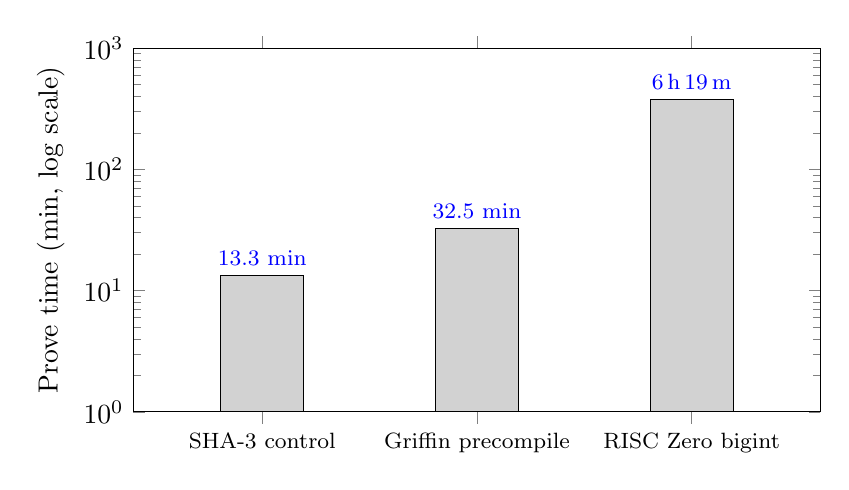
\begin{tikzpicture}
\begin{axis}[
  ybar,
  width=0.85\textwidth, height=6.2cm,
  ymode=log, ymin=1, ymax=1000,
  ylabel={Prove time (min, log scale)},
  symbolic x coords={SHA-3 control, Griffin precompile, RISC Zero bigint},
  xtick=data,
  x tick label style={font=\footnotesize},
  nodes near coords, point meta=explicit symbolic,
  every node near coord/.append style={font=\footnotesize},
  bar width=30pt, enlarge x limits=0.3,
]
\addplot+[draw=black, fill=gray!35] coordinates {
  (SHA-3 control, 13.28) [13.3 min]
  (Griffin precompile, 32.53) [32.5 min]
  (RISC Zero bigint, 379) [6\,h\,19\,m]
};
\end{axis}
\end{tikzpicture}
\caption{Prove time on the configurations that complete ($\lambda=80$, M5~Pro
24~GB, log scale). The bespoke Griffin precompile ($32.5$~min) is slower than the
SHA-3 control ($13.3$~min) at matched security, and RISC~Zero's \texttt{sys\_bigint}
route is slower again ($6$\,h\,$19$\,m); these are different hash and substrate
mechanisms, so the bars are not one artefact. The precompile-free baseline does not
complete (DNF, OOM at ${\approx}1$m$45$s) and so has no bar.}
\label{fig:prove-time}
\end{figure}

\paragraph{The honest reading.}
The with/without-precompile contrast is not a ratio of two finite times: without
the precompile the workload \emph{does not complete} on this hardware, and with
it the workload completes in $32.53$~minutes. The defensible claim is therefore
qualitative at the prove level (\emph{the precompile moves PLUM verification
from infeasible to feasible on consumer hardware}) and quantitative only at the
cycle level (\S\ref{ssec:attribution}). The two zkVMs are not directly comparable
here: SP1 runs the bespoke Griffin AIR, whereas RISC~Zero carries the field
arithmetic through \texttt{sys\_bigint} without a native Griffin chip
(\S\ref{ssec:griffin-air}); the large SP1-vs-RISC~Zero gap reflects that mechanism
difference and should not be read as a like-for-like substrate ranking. The SHA-3 control
isolates the hash family: the verification harness is identical except that every
Griffin-$\mathbb{F}_p^{192}$ sponge call is replaced by a SHA3-256 call computed in
software, so that the SHA-3 arm fires \emph{no} hash precompile and only the shared
\texttt{UINT256\_MUL} field-multiplication precompile remains active. It
shows that a workload using a \emph{standard} hash in software is markedly
cheaper than one using the algebraic hash PLUM requires through a bespoke chip,
which is the quantitative form of the arithmetic-mismatch argument of Section~\ref{sec:theoretical}. The
inversion is direct: the bespoke Griffin-$\mathbb{F}_p^{192}$ precompile
($32.53$~min) is about $2.45\times$ \emph{slower} at prove than the software
SHA-3 control ($13.28$~min) at matched $\lambda=80$. We read this as a genuine
property of the pipeline rather than a measurement artefact: in the deployed SP1
pipeline, arithmetising a $199$-bit-field algebraic hash through a custom AIR
costs more than a SHA-class hash the substrate already accelerates natively. What
the precompile bought us was a finite measurement; it did not buy a speedup.

\paragraph{Proof size, and why we do not re-measure it.}
Receipt size in SP1 is a property of the proof \emph{type}, not of the workload.
The runs above use SP1's default \emph{core} proof, whose size \emph{scales with
execution size}~\cite{succinct2025prooftypes}; the compact, on-chain-deployable
proof is instead the constant-size {SNARK} \emph{wrap} of that receipt, about
$260$~bytes for Groth16 over {BN254}, or $868$~bytes for
{PLONK}~\cite{succinct2025prooftypes}. Producing that wrap is exactly the step
that exhausts memory on the target hardware (the {PLONK} wrap was killed at
${\approx}20$~GB, \S\ref{ssec:resource-frontier}). On a $24$~GB machine, then, the
proof a deployer can actually generate is the large, shard-scaling core receipt;
the $260$-byte {SNARK} is a documented size the consumer-hardware frontier
prevents us from realising here. We therefore report the deployable figure as
documented and do not serialise the workload-dependent core receipt, whose byte
count is not the deployment-relevant number.

\subsection{The Circuit-SNARK Reference Point}\label{ssec:aurora-ref}

To situate the zkVM costs against the static-circuit regime they are meant to
escape, we measured the Aurora prover end-to-end over the BDEC R1CS on the same
hardware. This is the baseline the BDEC construction itself
uses~\cite{10.1007/978-981-96-0957-4_3}. We measure it directly rather than cite
it, so that the comparison is on our hardware rather than across machines.

\begin{table}[h]
\centering
\small
\begin{tabular}{lr}
\toprule
Quantity & Value \\
\midrule
Constraints (padded)        & $524{,}288$ \\
Prover time (setup $+$ prove) & $227.1$~s ($3.78$~min) \\
Verifier time               & $41.2$~s \\
Proof size                  & $688$~KB \\
Achieved security           & $107.5$ bits (target $128$) \\
Zero-knowledge              & disabled \\
\bottomrule
\end{tabular}
\caption{Aurora over the BDEC R1CS, M5~Pro 24~GB, single run. This is the
\emph{Loquat}-instantiated circuit over $\mathbb{F}_{p^2}$ ($127$-bit
base)~\cite{10.1007/978-981-96-0957-4_3}, \emph{not} the PLUM workload measured
elsewhere; the two are not a same-scheme comparison. Prover time includes Aurora
parameter setup but is not a recompile-time measurement (\S\ref{ssec:churn-eval}).
Achieved security $107.5$ bits, below the $128$ target. Verification \texttt{ACCEPT}.}
\label{tab:aurora-ref}
\end{table}

\paragraph{What this reference does and does not license.}
Two readings of this point are legitimate and one is not. \emph{Legitimate:} on this
hardware the static-circuit regime proves a BDEC credential statement in
minutes, against the zkVM's tens-of-minutes-to-infeasible
(Tables~\ref{tab:plum-verify},~\ref{tab:bdec}), so for a \emph{fixed} predicate
the static circuit is the faster prover, as one would expect from a specialised
encoding. \emph{Also legitimate:} this Aurora instance, like the zkVM succinct
receipt, is non-zero-knowledge here, so it does not by itself discharge BDEC's
anonymity requirement either. \emph{Not licensed:} reading
Table~\ref{tab:aurora-ref} as a like-for-like ``Aurora beats the zkVM'' verdict
on the same scheme, since it is Loquat over a $127$-bit field, whereas the zkVM
numbers are PLUM over a $199$-bit field, and it is timed without the
predicate-change cost that is the whole point of the update-churn comparison
(\S\ref{ssec:churn-eval}).

\subsection{Cost Attribution}\label{ssec:attribution}

To attribute the cost we use execute-mode cycle counts at $\lambda=128$, the
audience-relevant security level, where prove-mode is infeasible but cycle counts
remain machine-independent. Table~\ref{tab:ablation} reports the cumulative
effect of routing PLUM's field arithmetic through the host precompile, as an
ablation over the SHA-3-hasher verification path.

\begin{table}[h]
\centering
\small
\begin{tabular}{lrrr}
\toprule
Configuration (cumulative) & SP1 cycles & RISC~Zero cycles & $\Delta$ vs.\ baseline \\
\midrule
Baseline (\texttt{BigUint} emulation)        & 289{,}778{,}709 & 812{,}646{,}400 & n/a \\          % uint256 doc
$+$ field mul via host precompile            & 276{,}643{,}994 & n/a             & SP1 $-4.5\%$ \\
$+$ power as square-and-multiply             & 240{,}857{,}140 & n/a             & SP1 $-16.9\%$ \\
$+$ skip redundant reduction                 & 179{,}952{,}920 & 239{,}599{,}616 & SP1 $-37.9\%$, R0 $-70.5\%$ \\
\bottomrule
\end{tabular}
\caption{Cycle-level cost attribution, PLUM verification, SHA-3 hasher,
$\lambda=128$, \emph{execute mode}. Routing field arithmetic through the host
precompile (and removing redundant reductions) cuts $37.9\%$ of SP1 cycles and
$70.5\%$ of RISC~Zero cycles; RISC~Zero's larger reduction reflects its heavier
per-multiplication baseline ($6{,}625$ vs.\ $1{,}826$ cycles/mul).}
\label{tab:ablation}
\end{table}

\paragraph{Where the cost lives, and the parameter-set caveat.}
At $\lambda=128$ a single PLUM verification issues about $112{,}902$
$\mathbb{F}_p^{192}$ multiplication syscalls through the host precompile, as
counted in our own SP1 run log; this figure counts \emph{all} field
multiplications, the large majority of which occur \emph{inside} the Griffin
permutations rather than in the explicit field-arithmetic of the verifier (PLUM
\S4.2 reports only $\approx 10^3$ explicit verification multiplications). The
count is therefore consistent with the arithmetic-mismatch model: the cost is
dominated by the algebraic hash, whose internal field operations are routed
through the precompile. We caution explicitly against transferring the PLUM paper's
circuit-SNARK figure (that $91\%$ of \emph{R1CS constraints} are hash
work) directly to the zkVM cost model: that figure is a constraint count in a
different proving system, whereas Table~\ref{tab:ablation} is a RISC-V cycle
count. The qualitative conclusion (hash/field arithmetic dominates) agrees; the
exact share differs by cost model and is reported here in the zkVM's own units.
% [NEEDS DATA] a per-component split (Griffin vs FFT/sumcheck vs rest) would sharpen this.

\paragraph{Execute-mode delta for the Griffin precompile (PLUM-80).}
For the bespoke Griffin AIR specifically, the precompile-free versus
precompile-enabled execute-mode cycle counts differ by a factor of
$56.4\times$ at $\lambda=80$, the ratio of precompile-free to Griffin-AIR-enabled cycles on the Griffin arm; this is distinct from the $37.9\%/70.5\%$ of Table~\ref{tab:ablation}, a separate field-multiplication-reduction ablation reported at $\lambda=128$. % commit 2c1392b
We report this as an \emph{execute-mode cycle ratio} rather than a wall-clock speedup:
it is the machine-independent counterpart of the infeasible-to-feasible prove
transition of Table~\ref{tab:plum-verify}, and it is the figure that should be
cited when a single number is wanted, in place of any prove-time ``speedup,''
which is undefined when the baseline does not complete.

\subsection{PLUM-in-BDEC and the Consumer-Hardware Frontier}\label{ssec:frontier}

Moving from a single signature to the BDEC credential-generation relation
$R_{\mathsf{cre}}^{\mathsf{PLUM}}$ (two signature verifications under a hidden
user key; \S\ref{ssec:integration}), Table~\ref{tab:bdec} reports the
application-level result on RISC~Zero at $\lambda=80$.

\begin{table}[h]
\centering
\small
\begin{tabular}{l l p{3.2cm} p{4.6cm}}
\toprule
Workload & Mode & Cost & Outcome \\
\midrule
BDEC CreGen (PLUM, $\lambda=80$) & execute & $9.40\times10^{9}$ cyc, $\approx$65~s & both verifications accept \\ % plum_in_bdec doc
BDEC CreGen (PLUM, $\lambda=80$) & prove (succinct) & $\geq$15.6~h, peak RSS 11.24~GB & internal-verifier rejection (anomaly; \S\ref{ssec:cregen-anomaly}) \\ % risc0_prove_failure doc
\bottomrule
\end{tabular}
\caption{BDEC credential generation, RISC~Zero, $\lambda=80$, M5~Pro 24~GB.
Execute mode validates functional correctness ($9.4\times10^{9}$ cycles,
${\approx}4.69\times10^{9}$ per signature verification). The succinct-prove run
yielded no receipt; the cause was an internal-verifier rejection, not a resource
limit (\S\ref{ssec:cregen-anomaly}), and is not used as a feasibility result.}
\label{tab:bdec}
\end{table}

The execute-mode result establishes that the BDEC credential relation is
functionally correct end-to-end inside the zkVM: both signature verifications
accept, at $9.4\times10^{9}$ cycles. The prove-mode outcome requires care,
because it is \emph{not} the resource frontier it might first appear to be, and
we separate the two readings explicitly.

\subsubsection{An internal-verifier rejection rather than a resource frontier}\label{ssec:cregen-anomaly}
The succinct-prove run (RISC~Zero $3.0.3$, default \texttt{ProverOpts::succinct()}) terminated after $15.6$~hours with RISC~Zero's own
recursive aggregation step rejecting one of its intermediate segment proofs
(\texttt{verify segment / verification indicates proof is invalid}). This is
categorically different from running out of memory: peak resident memory was only
$11.24$~GB on the $24$~GB machine, with kernel free memory above $70\%$
throughout, so the machine was \emph{not} the limiting resource. An
internal-verifier rejection is a correctness anomaly; it tells us nothing about
deployability, and we therefore do \emph{not} report it as a frontier or fold it
into any feasibility claim. Its candidate causes are (i) an edge case in RISC~Zero's
recursion/segment-composition at a segment count ($9.4\times10^{9}$ guest cycles,
$\approx$$65\times$ the single-verification workload) beyond what public
benchmarks exercise; (ii) a non-ECC memory error over the long run; or (iii) a
precompile trace malformation that manifests only across a segment boundary,
which would bear on the chip--constraint equality (premise~(T2)) of Section~\ref{sec:security}. The segment count, segment size, and failing-segment index were not captured in
this run; a re-run with
segment-level diagnostics (\texttt{RUST\_LOG=risc0\_zkvm=debug}), intended to record those and to distinguish these causes, is the appropriate next
step; pending it, the anomaly is recorded as exactly that (an anomaly under
diagnosis), and the thesis's claims do not rest on it. The single PLUM
verification \emph{does} prove successfully on RISC~Zero
(Table~\ref{tab:plum-verify} reports the SP1 analogue; the RISC~Zero single-verify
prove completes and verifies). That is consistent with cause (i): the anomaly
appears at the larger segment count, and the verification logic itself proves clean.

\subsubsection{The genuine resource frontier}\label{ssec:resource-frontier}
The deployability frontier of this thesis rests on \emph{resource} failures,
which are unambiguous and independent of the anomaly above. Two are measured.
First, the PLONK zero-knowledge wrap of the standalone PLUM
single-signature-verification receipt (Cell~2 of Table~\ref{tab:plum-verify}, the
$32.53$-min prove, not CreGen or ShowCre) was killed under memory
pressure at ${\approx}82\%$ of the $24$~GB budget (${\approx}20$~GB of system
memory pressure at the kill; peak RSS ${\approx}17.8$~GB); this is the cost
specific to the anonymity-providing wrap, and it is the measured form of the
anonymity--deployability tension of Section~\ref{sec:security}. Second, and
separately, a \emph{non-zero-knowledge} baseline proof of a standardised-lattice
signature verification (an ML-DSA proxy: the $17$ NTT-domain polynomial
multiplications of $256$ coefficients modulo $q=8{,}380{,}417$ that dominate
ML-DSA-65 verification, proved as a baseline succinct STARK on SP1, not a
zero-knowledge wrap) reached a peak footprint of $82.7$~GB;
this is a substrate base-cost datum that \emph{strengthens but does not
instantiate} the tension, since it bears on the cost of proving any PQ
verification on this substrate, not on the zero-knowledge wrap specifically. These are the data points the frontier claim uses;
the positive feasibility anchor remains the PLUM single-verification prove of
Table~\ref{tab:plum-verify}, which completes in $32.53$~min. Table~\ref{tab:proof-mode}
summarises, for every proof mode attempted, whether a receipt is produced and whether
it is zero-knowledge and post-quantum.

\begin{table}[h]
\centering
\small
\renewcommand{\arraystretch}{1.2}
\begin{tabular}{@{}p{4.2cm}p{1.4cm}p{1.6cm}p{1.5cm}p{2.9cm}@{}}
\toprule
Proof mode (substrate / configuration) & Produced? & Zero-know\-ledge? & Post-quantum? & Resource outcome \\
\midrule
SP1, PLUM verify, Griffin precompile (\texttt{core}) & yes & no & yes & completes, $32.5$~min \\
SP1, PLUM verify, SHA-3 control (\texttt{core}) & yes & no & yes & completes, $13.3$~min \\
SP1, PLUM verify, Groth16/PLONK wrap & \textbf{no} & yes & \textbf{no} & OOM ${\approx}20$~GB \\
RISC~Zero, PLUM verify, \texttt{sys\_bigint} (succinct) & yes & no & yes & completes, $6$\,h\,$19$\,m \\
RISC~Zero, BDEC CreGen (succinct) & \textbf{no} & n/a & n/a & $\geq15.6$~h, internal-verifier rejection \\
Aurora, BDEC static (Loquat) & yes & no\textsuperscript{$\dagger$} & yes & completes, $3.78$~min \\
\bottomrule
\end{tabular}
\caption{Proof-mode feasibility matrix. The modes \emph{produced} on the target
hardware are not zero-knowledge; the only zero-knowledge mode the toolchain exposes
(row~3, a pairing wrap) is neither post-quantum nor produced within the memory
bound, which is the dual obstruction. \textsuperscript{$\dagger$}Aurora is
zero-knowledge-capable but the measured run had ZK disabled and ran below
$\lambda=128$. The SHA-3 row is a control, not a deployable PLUM variant.}
\label{tab:proof-mode}
\end{table}

\subsection{A Cost Model and the Substrate Crossover}\label{ssec:costmodel}
% The STUDY spine: turn point-measurements into a validated predictive model +
% the comparative viability (crossover) analysis. Anchors reconciled per-hasher
% (Griffin vs SHA-3) -- the ~33x gap between CreGen-Griffin (4.69e9/verify) and
% PLUM-verify-SHA3 (~1.4e8) IS the field-mismatch tax, NOT a basis error.

The measurements above are point observations; to answer ``what would this cost
at a configuration we did not run, and when is the flexible substrate the
rational choice,'' we fit a cost model to them and validate it against the points
we have. This is the analysis that converts the measurements from a benchmark
table into a basis for a deployment decision. The model is fitted and validated
in \emph{execute-mode cycle} counts; carrying it to prove-mode wall-clock assumes
the additive form survives recursion, memory pressure, segment aggregation, and
the zero-knowledge wrap, any of which can introduce nonlinearity, so the
prove-mode reading is an extrapolation, not a measured fit.

\subsubsection{An additive cost model for the BDEC relations}
Both BDEC relations are, at the cycle level, dominated by repeated
signature verifications (Section~\ref{ssec:cost-decomposition}): CreGen contains
two, and ShowCre contains $k+2$ for $k$ shown credentials. Writing
$C_{\mathsf{ver}}(\lambda,h)$ for the execute-mode cycle cost of one PLUM
verification at security level $\lambda$ under hasher $h$, and $C_0$ for the
fixed per-run overhead (input parsing and witnessing; the ledger-membership,
revocation, and disclosure checks are performed by the relying party outside the
proof), the model is
\begin{align}
  C_{\mathsf{CreGen}}(\lambda,h) &\approx 2\,C_{\mathsf{ver}}(\lambda,h) + C_0,
  \label{eq:cost-cregen}\\
  C_{\mathsf{ShowCre}}(k,\lambda,h) &\approx (k+2)\,C_{\mathsf{ver}}(\lambda,h) + C_0,
  \label{eq:cost-showcre}
\end{align}
The model is deliberately linear in the verification count, because the cost
decomposition of Section~\ref{ssec:cost-decomposition} shows that everything else
in the proof is dominated by the $\Theta(k)$ algebraic-hash work inside the
verifications; the ledger-membership, revocation, and disclosure checks do not
enter the proving cost, as the relying party performs them outside the proof.

\subsubsection{Validation against the measured points}
The model is falsifiable against the two BDEC points we measured. The strongest
internal check is CreGen: Equation~\eqref{eq:cost-cregen} predicts the two
verifications should each cost $\approx C_{\mathsf{ver}}$ and together dominate
the trace. The measurement bears this out directly: the two verifications cost
$4.69\times10^{9}$ cycles \emph{each} (the two within $0.01\%$ of \emph{each
other}), their sum $9.38\times10^{9}$ accounting for $\approx99.8\%$ of the
$9.40\times10^{9}$ total
(Table~\ref{tab:bdec}); so for the Griffin hasher at $\lambda=80$,
$C_{\mathsf{ver}}(\textsf{80},\textsf{Griffin})\approx 4.69\times10^{9}$ cycles
and $C_0$ is small. We caution that this single relation validates the
\emph{linearity} and the \emph{verification-dominance}, not the absolute
constant at other $(\lambda,h)$; the $k=14$ projection below is labelled as such.

\paragraph{The hasher gap measures the tax.}
A single PLUM verification is markedly cheaper with the SHA-3 hasher control than
with the Griffin algebraic hash, an order-of-magnitude separation that is the
field-mismatch tax of Section~\ref{sec:theoretical} quantified at the
verification level. We state the gap only as indicative: the two figures we have
to hand sit at different security levels (the Griffin $4.69\times10^{9}$ at
$\lambda=80$, the SHA-3 control in the $\lambda=128$ ablation of
Table~\ref{tab:ablation}), and our own non-comparability rule forbids dividing
across that seam to produce a single ratio. The qualitative conclusion (that the
algebraic hash is the tax-bearing component while the field arithmetic is not, so
$C_{\mathsf{ver}}$ must be reported per hasher) holds regardless of the exact
multiplier. The precompile narrows
this gap (Table~\ref{tab:ablation}); closing it entirely is what a native
Griffin AIR on the proving path would buy.

\paragraph{ShowCre execute-mode cost (measured at $k=1,2$).}
The ShowCre relation is realised by the guest
\texttt{bdec\_showcre\_plum\_griffin}, the $k+2$ generalisation of the CreGen
guest, and measured in execute mode at the two running examples. At $k=1$ (the
$\phi_1$ workload) ShowCre executes in $1.41\times10^{10}$ cycles, and at $k=2$
(the $\phi_2$ workload) in $1.88\times10^{10}$ cycles, each with all $k+2$
verifications accepting. Both agree with Equation~\eqref{eq:cost-showcre} at
$C_{\mathsf{ver}}(\textsf{80},\textsf{Griffin})\approx 4.69\times10^{9}$: the
per-verification cost is constant at $\approx 4.69\times10^{9}$ cycles across
CreGen and both ShowCre instances, so the additive $(k+2)\,C_{\mathsf{ver}}$ form
is measured rather than assumed. Applying the same measured constant to a stress-test disclosure-set size, well
beyond the running examples ($k=1,2$) and the $k\le 4$ design target, projects
$\approx 7.5\times10^{10}$ cycles at $k=14$. A direct $k=14$ execute run does not reach this
projection: the $16$ accumulated verifications exhaust the guest's default
non-reclaiming bump allocator before the cycle count completes, an in-guest memory
limit distinct from the prover-side memory frontier and clearable only by the
reclaiming allocator at additional cycle cost. The $k=1$ and $k=2$ executions are
correct and their cost is measured; the zero-knowledge \emph{proof}, however,
rests on the same anonymity-providing wrap whose memory exhaustion is the
consumer-hardware frontier of \S\ref{ssec:resource-frontier} (the ${\approx}20$~GB
PLONK wrap; $82.7$~GB for the standardised-lattice baseline). A zero-knowledge
proof of ShowCre at any $k\ge 1$ is therefore bounded by that wrap frontier, not
by the CreGen prove anomaly (an internal-verifier rejection, not a resource limit;
\S\ref{ssec:cregen-anomaly}). More memory would clear the resource bound, but a
post-quantum-anonymous proof additionally requires a post-quantum-sound wrap
(Section~\ref{sec:security}).

\subsubsection{The substrate crossover}\label{sssec:crossover}
The decision a deployer faces (Section~\ref{sec:discussion}) is not about which
substrate is faster per proof, since the static circuit wins that in any case. It
is about which substrate is cheaper over a deployment \emph{lifetime} during which
the predicate changes. Let the lifetime
contain $P$ proof generations and $U$ localised predicate changes. Amortised
total cost is, schematically,
\begin{align}
  \text{static:}\quad & U\cdot R_{\mathsf{static}} + P\cdot t^{P}_{\mathsf{static}},
  \label{eq:static-cost}\\
  \text{zkVM:}\quad & U\cdot 0 + P\cdot t^{P}_{\mathsf{zkVM}},
  \label{eq:zkvm-cost}
\end{align}
where $R_{\mathsf{static}}$ is the per-change recompilation cost and $t^{P}$ is
per-proof time. We isolate $R_{\mathsf{static}}$ directly (\S\ref{ssec:churn-eval}):
for the full BDEC R1CS it is R1CS construction ($\approx 0.2$~s) plus Aurora
parameter setup (measured at $\approx 3\,\mu$s, because Aurora is
non-preprocessing), so $R_{\mathsf{static}}\approx 0.3$~s. The multi-minute figure
of Table~\ref{tab:aurora-ref} is the per-\emph{proof} prover, not the per-change
recompile, and does \emph{not} enter $R_{\mathsf{static}}$. The zkVM's update term is zero
(Table~\ref{tab:churn}). The static regime is cheaper only while
\[
  U\cdot R_{\mathsf{static}} < P\,\bigl(t^{P}_{\mathsf{zkVM}}-t^{P}_{\mathsf{static}}\bigr),
\]
i.e.\ while the relation-change rate $U/P$ stays below a crossover
\[
  \Bigl(\tfrac{U}{P}\Bigr)^{\!*} \;=\; \frac{t^{P}_{\mathsf{zkVM}}-t^{P}_{\mathsf{static}}}{R_{\mathsf{static}}}.
  \label{eq:crossover}
\]
The measured $R_{\mathsf{static}}\approx 0.3$~s is decisive, and it cuts
\emph{against} a naive flexibility argument. Because $R_{\mathsf{static}}$ is
sub-second while the zkVM's per-proof penalty exceeds the static prover's
($t^{P}_{\mathsf{zkVM}}>t^{P}_{\mathsf{static}}$ even granting the cross-scheme seam
of \S\ref{ssec:aurora-ref}: static Loquat-$\mathbb{F}_{p^{127}}$, zkVM
PLUM-$\mathbb{F}_{p}$), the crossover $\bigl(U/P\bigr)^{*}$ of
Eq.~\ref{eq:crossover} is on the order of thousands of relation changes per proof,
a regime no realistic deployment reaches. \textbf{Against a transparent,
non-preprocessing argument such as Aurora, the zkVM thus has no wall-clock
flexibility advantage:} both regimes rebuild a sub-second artefact per change, and
the zkVM is then dearer per proof. Recompile wall-clock does not capture the
genuine per-change cost of the static regime; that cost is the \emph{re-audit and
engineering} footprint of a new relation-specific circuit
(Table~\ref{tab:churn}, $N_{\mathsf{circ}}/N_{\mathsf{param}}$). A \emph{wall-clock} flexibility advantage would appear only
against a \emph{preprocessing} argument (Groth16~\cite{groth2016}, Marlin~\cite{chiesa2020marlin}, or circuit-specific
PLONK~\cite{gabizon2019plonk}), whose per-circuit key generation makes $R_{\mathsf{static}}$ large, and
Aurora, the BDEC baseline, is not such a system. We therefore report the
flexibility result as \emph{qualitative} (the regeneration footprint of
Table~\ref{tab:churn}) together with this measured wall-clock caveat, rather than
as a numeric crossover that favours the zkVM.

\subsection{Update Churn}\label{ssec:churn-eval}

Table~\ref{tab:churn} enumerates the regeneration footprint of
Definition~\ref{def:update-churn} for the three localised changes of
\S\ref{ssec:update-churn}, using $\phi_1\!\to\!\phi_2$
(par.~\ref{par:phi-examples}) as the presentation-change instance. Here
$\phi_1\!\to\!\phi_2$ is a presentation-\emph{structure} change: it moves the
credential count from $k{=}1$ to $k{=}2$, altering the relation
$R_{\mathsf{show}}^{\Sig}$ and hence the static R1CS. A presentation \emph{policy}
change at fixed structure (e.g.\ retuning a threshold the verifier checks on the
disclosed attributes) is handled verifier-side and triggers no regeneration on
either substrate, so the rows below measure structural changes.

\begin{table}[h]
\centering
\small
\begin{tabular}{lcccc}
\toprule
& \multicolumn{2}{c}{Static circuit (Aurora)} & \multicolumn{2}{c}{zkVM} \\
\cmidrule(lr){2-3}\cmidrule(lr){4-5}
Localised change & $N_{\mathsf{circ}}$ & $N_{\mathsf{param}}$ & $N_{\mathsf{circ}}$ & $N_{\mathsf{param}}$ \\
\midrule
Presentation change ($\phi_1\!\to\!\phi_2$, $k{:}1{\to}2$) & $\geq 1$ & $\geq 1$ & $0$ & $0$ \\
Signature swap (Loquat $\to$ PLUM)              & $\geq 1$ & $\geq 1$ & $0$ & $0$ \\
Security retune ($\lambda{=}80\to128$)          & $\geq 1$ & $\geq 1$ & $0$ & $0$ \\
\bottomrule
\end{tabular}
\caption{Circuit/parameter regeneration footprint ($N_{\mathsf{circ}},N_{\mathsf{param}}$
of Definition~\ref{def:update-churn}). The static-circuit regime regenerates and
re-audits its R1CS and constraint-dependent parameters on every localised change;
the zkVM absorbs all changes as guest-program edits, leaving the universal relation
unchanged ($N_{\mathsf{circ}}=N_{\mathsf{param}}=0$). The components
$N_{\mathsf{src}},N_{\mathsf{audit}}$ are not integer-countable and are discussed in
prose.}
\label{tab:churn}
\end{table}

\paragraph{Structural separation, and the measured recompile cost.}
The structural separation in Table~\ref{tab:churn} is established by
construction: a zkVM's relation is fixed to the ISA, so a presentation-structure
or signature change is absorbed as a source edit
($N_{\mathsf{circ}}=N_{\mathsf{param}}=0$) with no recompilation. \emph{Both}
components of the static side are now measured, and the result overturns the
earlier conjecture that recompilation is expensive. R1CS
\emph{construction} from the BDEC relation is sub-second ($0.18$~s at
Loquat-$\lambda{=}80$, $0.24$~s at $\lambda{=}128$, three runs each). The Aurora
\emph{parameter setup} that a relation change forces to recompute is, measured
directly, about $3\,\mu$s (the runner reports $t_{\mathrm{setup}}=0.003$~ms at the
full $2^{19}$-padded BDEC R1CS), because Aurora is \emph{non-preprocessing}: it has
no per-circuit indexer. The prover's low-degree-encoding FFTs (its dominant step) run \emph{per proof},
not per relation change, and so do not enter $R_{\mathsf{static}}$. Hence $R_{\mathsf{static}}\approx 0.3$~s for the whole BDEC
relation. A $\phi_1\!\to\!\phi_2$ change alters only the credential count and does
not enlarge the microsecond parameter setup, so this bound also holds for the
per-presentation delta; a $k$-parameterised emitter would refine the
R1CS-construction term but cannot move the dominant conclusion, namely that for a
transparent non-preprocessing argument the per-change recompile is sub-second.
Consequently the zkVM's wall-clock flexibility advantage over Aurora is negligible,
and the static regime's real per-change cost is the \emph{re-audit} of a new
circuit (Table~\ref{tab:churn}) rather than recompile time.
% [MEASURED 2026-06-05] R_static ~0.3s (param-setup ~3us measured, non-preprocessing; the FFTs are per-proof, not per-recompile). docs/r_static_finding_20260605.md. Sako [10:39],[17:10].

\paragraph{The advantage is conditional on the baseline's preprocessing model.}
The negligible recompile cost above is a property of Aurora's \emph{non-preprocessing}
structure; it does not generalise to static circuits at large. A \emph{preprocessing} (holographic)
transparent argument such as Fractal~\cite{cryptoeprint:2019/1076} must instead build
a per-circuit index, and that index is exactly what a relation change forces to
regenerate. Timing Fractal's indexer (its \texttt{fractal\_snark\_indexer} stage) in
isolation on the same Loquat-BDEC R1CS over the $127$-bit field (the same harness as
\S\ref{ssec:aurora-ref}; ${\approx}107$-bit achieved, zero-knowledge disabled; a Loquat
proxy for PLUM) gives the contrast of Table~\ref{tab:rstatic-fractal}: Aurora's
parameter setup is microseconds and flat in circuit size, whereas Fractal's holographic
indexer grows superlinearly and, at the $2^{19}$-padded BDEC size, is killed under
memory pressure mid-indexer (during a $2^{27}$-element FFT) before returning.

\begin{table}[h]
\centering
\small
\begin{tabular}{lcc}
\toprule
R1CS size (constraints) & Aurora $R_{\mathsf{static}}$ (param.\ setup) & Fractal $R_{\mathsf{static}}$ (indexer) \\
\midrule
$2^{10}$ ($1{,}024$)          & $0.0021$~ms & $0.86$~s \\
$2^{12}$ ($4{,}096$)          & $0.0023$~ms & $3.74$~s \\
$2^{14}$ ($16{,}384$)         & $0.0025$~ms & $18.5$~s \\
$2^{19}$ (BDEC, $524{,}288$)  & $0.0029$~ms & OOM-killed at ${\approx}33$~min \\
\bottomrule
\end{tabular}
\caption{Per-change recompile cost $R_{\mathsf{static}}$ for a non-preprocessing
(Aurora) versus a preprocessing (Fractal) transparent argument, same Loquat-BDEC R1CS
($127$-bit field), M5~Pro 24~GB. Aurora has no per-circuit indexer
($R_{\mathsf{static}}$ flat at ${\sim}\mu$s); Fractal's indexer is superlinear and
exceeds $24$~GB at the BDEC size (OOM mid-indexer). The zkVM regenerates no circuit.}
\label{tab:rstatic-fractal}
\end{table}

\noindent The flexibility reading is therefore \emph{conditional on the static
baseline's preprocessing model}: the zkVM's wall-clock recompile advantage is
negligible against a non-preprocessing argument (Aurora) and large against a
preprocessing one (Fractal), where at the BDEC circuit size the baseline's per-circuit
indexing is itself infeasible on the target hardware. The same-scheme and field seam
of \S\ref{ssec:aurora-ref} applies throughout (a Loquat proxy, not PLUM), and a
smaller folding parameter than the Aurora-matched $\mathsf{RS}=5$ might let the Fractal
indexer fit and yield a finite but still large $R_{\mathsf{static}}$.

\subsection{What the Measurements Establish}\label{ssec:scorecard}

We close by reading the measurements back against the cost framework of
Section~\ref{sec:theoretical}.

\paragraph{Feasibility and the field-mismatch tax.}
Without the precompile a single PLUM verification does not complete on the target
hardware (out-of-memory at ${\approx}1\mathrm{m}45\mathrm{s}$,
Table~\ref{tab:plum-verify}); with it the verification completes in $32.53$~min.
At the cycle level the bespoke Griffin precompile removes a $56.4\times$ factor at
$\lambda=80$ (\S\ref{ssec:attribution}) and $37.9\%$/$70.5\%$ of SP1/RISC~Zero
cycles at $\lambda=128$ (Table~\ref{tab:ablation}). This is the field-mismatch tax
of Definition~\ref{def:fmt} made concrete: the precompile turns an infeasible
workload into a feasible one, and the residual cost is what the rest of the
evaluation measures. The with/without contrast at the prove level is an
infeasible-to-feasible transition rather than a finite ratio (\S\ref{ssec:headline}); the
factors above are cycle-level and single-verification, and we do not promote them
to a CreGen-relation prove speedup we did not run.

\paragraph{Where the cost lives.}
The cost attribution of \S\ref{ssec:attribution} bears out the decomposition of
\S\ref{ssec:cost-decomposition}: the dominant term is the algebraic hash, whose
internal field operations account for the large majority of the
$\mathbb{F}_p^{192}$ multiplications, not the explicit verifier field arithmetic.
We report this in the zkVM's own cycle units and caution against transferring
PLUM's circuit-SNARK ``$91\%$ of constraints are hash'' figure to the cycle model.

\paragraph{Per-proof cost against the static circuit.}
For a \emph{fixed} predicate the specialised static circuit is the faster prover,
as expected from a specialised encoding: Aurora proves the BDEC circuit in
$3.78$~min (Table~\ref{tab:aurora-ref}) against $32.53$~min for precompiled PLUM
verification (Table~\ref{tab:plum-verify}). The prove times do \emph{not}
converge; but the two points are not the same scheme (Loquat over
$\mathbb{F}_{p^2}$ versus PLUM over its $199$-bit prime field, \S\ref{ssec:aurora-ref}),
so we state the gap as indicative, and the comparison the thesis turns on is the
deployment-lifecycle one below rather than the per-proof one. Closing the per-proof gap
requires a same-scheme measurement: either running Loquat verification inside the
zkVM to match the static Loquat/Aurora point, or building an $\mathbb{F}_p$
($199$-bit) Aurora harness to run PLUM statically (the current Aurora harness is
$\mathbb{F}_{p_{127}}$-only); we identify this as the required follow-up experiment.

\paragraph{Update churn.}
The structural separation of Definition~\ref{def:update-churn} holds by
construction (Table~\ref{tab:churn}): every localised change regenerates at least
one circuit and one parameter set on the static side and none on the zkVM side,
provided the change does not alter a precompiled primitive or its field; a change
to the hash family or field width regenerates the Griffin AIR and so incurs
$N_{\mathsf{circ}}\ge1$ on the zkVM side too (Definition~\ref{def:update-churn}).
The recompile wall-clock of the static side is now measured
($R_{\mathsf{static}}\approx 0.3$~s; \S\ref{ssec:churn-eval}) and is sub-second
because Aurora is non-preprocessing; the gap that remains is a \emph{same-scheme}
per-proof static prover time (\S\ref{ssec:aurora-ref}) rather than the recompile,
our static point being Loquat and our zkVM point PLUM.

\paragraph{The zero-knowledge frontier.}
The base proof completes; what binds on consumer hardware is the zero-knowledge
wrap. A PLONK wrap of a PLUM proof exhausts memory (the cost specific to the
anonymity-providing wrap), which is the measured form of the
anonymity--deployability tension of Section~\ref{sec:security}; a
\emph{non-zero-knowledge} standardised-lattice baseline separately reaches
$82.7$~GB peak (\S\ref{ssec:resource-frontier}), a substrate base-cost that
strengthens but does not instantiate that tension. The frontier claim rests on
this resource-failure evidence, \emph{not} on the CreGen prove anomaly of
\S\ref{ssec:cregen-anomaly}, which is an internal-verifier rejection.

\subsection{Threats to Validity}\label{ssec:threats}

\begin{itemize}
  \item \textbf{Single-run timings.} The prove-mode wall-clock figures
  (Tables~\ref{tab:plum-verify}, \ref{tab:aurora-ref}) are single runs; we report
  no variance, and thermal or scheduling noise on a laptop-class machine over
  multi-minute runs is not characterised.
  \item \textbf{Thermal throttling.} Runs are on a laptop-class M5~Pro; sustained
  multi-minute proving may throttle, which would inflate wall-clock relative to a
  thermally-unconstrained host.
  \item \textbf{Hardware/OS-string provenance.} The reported platform string is
  from \texttt{sysctl}; we have not cross-checked every sub-component against an
  independent inventory.
  \item \textbf{Incomplete statement binding.} The RISC~Zero prototype does not
  yet bind the receipt journal to the public statement $(c,h,\mathsf{ppk})$
  (Section~\ref{sec:system}); until it does, an accepting receipt is a functional
  benchmark and not a statement-bound credential proof, which is a security gap and not a timing one.
  \item \textbf{Unresolved CreGen prove anomaly.} The $15.6$-hour BDEC
  credential-generation prove run ended in an internal-verifier rejection
  (\S\ref{ssec:cregen-anomaly}), not a resource limit; it is a single run with
  undetermined cause, no claim of this thesis rests on it, and a
  segment-diagnostic re-run is required before any statement about it. It is
  explicitly \emph{not} part of the resource frontier
  (\S\ref{ssec:resource-frontier}).
  \item \textbf{Parameter-set seam.} Prove-mode wall-clock is at $\lambda=80$;
  cycle attribution is at $\lambda=128$. The two are never combined into one
  figure, but a reader must track which is which; the tables are labelled
  accordingly.
  \item \textbf{Non-uniform precompile.} SP1 uses the bespoke Griffin AIR;
  RISC~Zero uses \texttt{sys\_bigint}. Cross-zkVM numbers reflect this mechanism
  difference and are not a like-for-like substrate comparison.
  \item \textbf{Constraint-level soundness of the Griffin AIR is empirically
  supported, not proved} (the chip--constraint equality, premise~(T2), of Section~\ref{sec:security}); the cost figures assume
  the chip computes the reference permutation, tested on $256$ random vectors but
  not verified at the constraint level.
  \item \textbf{Control vs.\ deployable.} The SHA-3 arm is a diagnostic control;
  it is not a secure PLUM variant and its timing is not a deployment claim.
\end{itemize}

\subsection{Summary}\label{ssec:eval-summary}
On consumer hardware, the precompile suite moves PLUM verification from infeasible
to feasible (Table~\ref{tab:plum-verify}), with the cost dominated by
large-field/algebraic-hash arithmetic and reduced by $37.9$--$70.5\%$ at the cycle
level (Table~\ref{tab:ablation}); the full BDEC credential relation is functionally
correct in execute mode, while its succinct prove ended in an internal-verifier
rejection categorically distinct from the resource frontier (Table~\ref{tab:bdec},
\S\ref{ssec:cregen-anomaly}), the binding consumer-hardware frontier being the
zero-knowledge wrap (\S\ref{ssec:resource-frontier}); and the zkVM regime is structurally free of the
update churn that the static-circuit regime incurs on every localised change
(Table~\ref{tab:churn}). The one comparison the data does not yet settle is a \emph{same-scheme} per-proof prover time across the two substrates; the static-circuit recompile wall-clock is now measured ($R_{\mathsf{static}}\approx 0.3$~s) and is not the bottleneck. The next chapter takes up what these results mean for the deployment decision and which questions they leave open.
